\newpage
	\section{G} \label{sec:G}
		\subsection{GESTIONE DELLA CONFIGURAZIONE} \index{Gestione della configurazione} \label{gestioneconfigurazione}
		Processo di supporto implicato dall'\underline{\hyperref[analisideirequisiti]{Analisi dei requisiti}} che è un documento collaborativo in cui ognuno ha una determinata parte e non c'è confusione.

		\subsection{GESTIONE DEI CAMBIAMENTI} \index{Gestione dei cambiamenti} \label{gestionecambiamenti}
		Processo di supporto implicato dall'\underline{\hyperref[analisideirequisiti]{Analisi dei requisiti}} perchè l'analisi dei requisiti non è un'attività libera da vincoli. Ogni cambiamento deve avere un resoconto. \\
		Valuta la fattibilità tecnica e l'impatto sul progetto.

		\subsection{GESTIONE DEI REQUISITI}	\index{Gestione dei requisiti} \label{gestionerequisiti}
		Attività da svolgere per l'\underline{\hyperref[analisideirequisiti]{Analisi dei requisiti}}. Prevede l'identificazione e la \underline{\hyperref[classificazione]{classificazione}} dei \underline{\hyperref[requirements]{requisiti}}:
		\begin{itemize}
			\item Identificatore unico
			\item Numerazione sequenziale basata sulla struttura del documento
			\item Organizzazione secondo la coppia [\texttt{CATEGORIA}, \texttt{NUMERO}]
		\end{itemize}
		Avviene inoltre la \underline{\hyperref[gestionecambiamenti]{gestione dei cambiamenti}} e la \underline{\hyperref[tracciamento]{tracciabilità}} (\textit{requisiti} in rapporto a \textit{parti della specifica} in rapporto a \textit{componenti del sistema}).

		\subsection{GESTIONE DEI RISCHI} \index{Gestione dei rischi} \label{gestionerischi}
		Fa parte della \underline{\hyperref[gestioneprogetto]{gestione di progetto}}. Prevede:
			\begin{itemize}
				\item Identificazione dei rischi nel progetto, nel prodotto e nel mercato
				\item Analisi della probabilità di occorrenza e conseguenze possibili
				\item \underline{\hyperref[pianificazione]{Pianificazione}}, ovvero come evitare i rischi e mitigarne gli effetti
				\item Controllo, ovvero prestare continua attenzione tramite rilevazione di indicatori e raffinamento delle strategie
			\end{itemize}
		\begin{figure}[H]
			\centering
			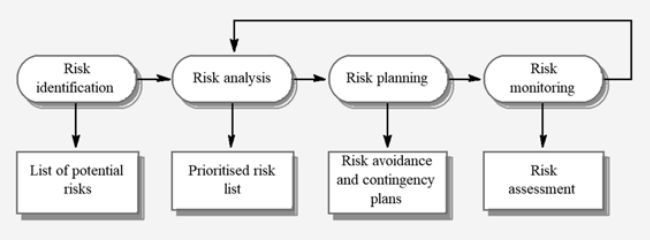
\includegraphics[width=0.8\textwidth]{img/rischi}
			\caption{Schema della gestione dei rischi.}
		\end{figure}



		\subsection{\emph{GESTIONE DI PROGETTO}} \index{Gestione di progetto} \label{gestioneprogetto}	%V.I.
		La gestione di progetto prevede:
			\begin{itemize}
				\item L'istanziazione di processi nel progetto secondo degli \underline{\hyperref[standard]{standard di processo}}
				\item La stima di costi e risorse necessarie tramite \underline{\hyperref[cocomo]{CoCoMo}}. I fattori di influenza per le stime sono:
				\begin{itemize}
					\item Dimensione del progetto
					\item Esperienza del dominio
					\item Familiarità con le tecnologie
					\item Produttività dell'ambiente di lavoro
					\item \underline{\hyperref[qualita]{Qualità}} attesa
				\end{itemize}
				\item \underline{\hyperref[pianificazione]{Pianificazione}} (partendo dall'obiettivo, quindi all'indietro, non dall'inizio) di attività con conseguente assegnamento alle varie persone
				\item Il controllo delle attività e la verifica dei risultati
			\end{itemize}
		In questo contesto ogni persona assume un certo \underline{\hyperref[ruoli]{ruolo}} e ad ogni ruolo viene assegnata un'attività (da notare che spesso molte risorse possono essere impegnate su più progetti). La gestione di progetto prevede anche la  \underline{\hyperref[gestionequalita]{Gestione di Qualità}} e un \underline{\hyperref[piano]{Piano di Progetto}}. \\
		I principali \textit{fattori di successo} di un progetto sono:
		\begin{itemize}
			\item Il coinvolgimento del cliente
			\item Il supporto della direzione esecutiva
			\item La definizione chiara dei requisiti
			\item Una pianificazione corretta
			\item Delle aspettative realistiche
			\item Un personale competente
		\end{itemize}
		Mentre i primi \textit{fattori di fallimento} sono:
		\begin{itemize}
			\item Dei requisiti incompleti
			\item Il mancato coinvolgimento del cliente
			\item La mancanza di risorse
			\item Delle aspettative non realistiche
			\item La mancanza di supporto  esecutivo
		\end{itemize}

		\subsection{GESTIONE DI QUALITÀ}  \index{Gestione di qualità} \label{gestionequalita}
		È una funzione di più recente introduzione aziendale. La \underline{\hyperref[qualita]{qualità}} riguarda qui sia i prodotti che i processi e interessa sia committente che la direzione aziendale. \\
		La garanzia di qualità produce confidenza, ma richiede l'applicazione rigorosa dei processi adottati e la loro \underline{\hyperref[manutenzione]{manutenzione}} migliorativa (ciclo di \underline{\hyperref[pdca]{PDCA}}).
